% Paytm Hisaab -- Build for India pitch deck
%
% Compile with XeLaTeX (needed for the rupee sign and the Kannada line):
%
%   cd pitch
%   xelatex hisaab-pitch.tex                          -> hisaab-pitch.pdf
%
% Fonts: Segoe UI + Nirmala UI (both ship with Windows). On another OS the
% deck still builds; it falls back to the default sans and drops the
% Kannada styling.
\documentclass[aspectratio=169,10pt]{beamer}

\usepackage{fontspec}
\usepackage{tikz}
\usepackage{booktabs}
\usepackage{array}
\newcolumntype{L}[1]{>{\raggedright\arraybackslash}p{#1}}
\usepackage{graphicx}
\usetikzlibrary{calc,positioning,arrows.meta}

\graphicspath{{./}{../}}

% ---------- fonts ----------
\IfFontExistsTF{Segoe UI}{\setsansfont{Segoe UI}}{}
\IfFontExistsTF{Nirmala UI}{%
  \newfontfamily\kn[Script=Kannada]{Nirmala UI}}{%
  \newcommand{\kn}{}}
\renewcommand{\familydefault}{\sfdefault}

% ragged, unhyphenated text inside the narrow cards
\hyphenpenalty=10000
\exhyphenpenalty=10000
\emergencystretch=3em
\hbadness=10000

% ---------- palette (taken from the product mock) ----------
\definecolor{navy}{HTML}{002970}
\definecolor{ptmcyan}{HTML}{00BAF2}
\definecolor{ink}{HTML}{0F172A}
\definecolor{muted}{HTML}{64748B}
\definecolor{good}{HTML}{15803D}
\definecolor{bad}{HTML}{DC2626}
\definecolor{amber}{HTML}{B45309}
\definecolor{tint}{HTML}{EAF4FD}
\definecolor{hairline}{HTML}{DBE7F3}

% ---------- theme ----------
\usetheme{default}
\usecolortheme{default}
\setbeamertemplate{navigation symbols}{}
\setbeamersize{text margin left=0.85cm,text margin right=0.85cm}
\setbeamercolor{normal text}{fg=ink,bg=white}
\setbeamercolor{frametitle}{fg=navy}
\setbeamercolor{structure}{fg=navy}
\setbeamerfont{frametitle}{size=\large,series=\bfseries}
\setbeamerfont{framesubtitle}{size=\scriptsize}
\setbeamercolor{framesubtitle}{fg=muted}
\setbeamertemplate{frametitle}{%
  \vspace{0.30cm}%
  \usebeamerfont{frametitle}\usebeamercolor[fg]{frametitle}\insertframetitle%
  \ifx\insertframesubtitle\empty\else{\\[-0.15em]\usebeamerfont{framesubtitle}\usebeamercolor[fg]{framesubtitle}\insertframesubtitle}\fi%
  \\[0.1em]{\color{ptmcyan}\rule{1.2cm}{2pt}}\par\vspace{-0.15em}%
}
\setbeamertemplate{footline}{%
  \hbox{\begin{beamercolorbox}[wd=\paperwidth,ht=1.9ex,dp=1.1ex,leftskip=0.85cm,rightskip=0.85cm]{}%
  {\scriptsize\color{muted}Paytm Hisaab\hfill\insertframenumber}%
  \end{beamercolorbox}}%
}
\setbeamerfont{itemize/enumerate body}{size=\normalsize}

% ---------- helpers ----------
\newcommand{\hi}[1]{{\color{navy}\bfseries #1}}
\newcommand{\red}[1]{{\color{bad}\bfseries #1}}
\newcommand{\grn}[1]{{\color{good}\bfseries #1}}
\newcommand{\sub}[1]{{\color{muted}#1}}
\newcommand{\qm}[1]{``#1''}
\newcommand{\bignum}[2]{{\color{navy}\fontsize{22}{24}\selectfont\bfseries #1}\\[0.1em]{\scriptsize\color{muted}#2}}
% a soft rounded card:  \card{width}{body}
\newcommand{\card}[2]{\begin{tikzpicture}%
  \node[rounded corners=4pt,fill=tint,inner sep=8pt,text width=#1,align=left]{#2};%
  \end{tikzpicture}}
% an outlined card:  \ocard{colour}{width}{body}
\newcommand{\ocard}[3]{\begin{tikzpicture}%
  \node[rounded corners=4pt,fill=white,draw=#1,line width=0.9pt,inner sep=8pt,text width=#2,align=left]{#3};%
  \end{tikzpicture}}

\begin{document}

% ============================================================ 1. TITLE
{\setbeamertemplate{footline}{}
\begin{frame}[plain]
\vspace{0.9cm}
\begin{center}
{\fontsize{38}{42}\selectfont\bfseries\color{navy}Paytm\;\color{ink}Hisaab}\\[0.45em]
{\Large\color{muted}Every rupee, on your side.}\\[0.9em]
{\color{ptmcyan}\rule{2.8cm}{2.5pt}}\\[0.9em]
{\large\color{ink}The teammate that accounts for a merchant's money when an authority}\\[0.15em]
{\large\color{ink}demands an explanation, and answers on their behalf inside the deadline.}\\[1.3em]
{\small\color{muted}Paytm Build for India \;$\cdot$\; Bengaluru, 19 September 2026 \;$\cdot$\; Track 3: Autonomous AI Teammates}
\end{center}
\end{frame}}

% ============================================================ 2. THE FREEZE
\begin{frame}{09:30 on a Tuesday}{The payments stop going through}
\vspace{0.15cm}
\begin{columns}[T]
\begin{column}{0.52\textwidth}
\vspace{0.15cm}
No message. No reason. No reference number.\\[0.6em]
She sold someone 12 kg of onions. That customer was three layers downstream of a fraud victim in another state.\\[0.6em]
She is not named in the FIR. \hi{339 payments} came into her account that week, and she cannot tell you which one is the problem.\\[0.6em]
Her supplier payment is due today.
\end{column}
\begin{column}{0.44\textwidth}
\vspace{0.6cm}
\ocard{bad}{5.4cm}{\centering
  {\color{muted}\scriptsize The disputed amount is}\\[0.5em]
  {\fontsize{26}{30}\selectfont\bfseries\color{bad}₹4,200}\\[0.6em]
  {\color{muted}\scriptsize The whole account is held.}}
\end{column}
\end{columns}
\vspace{0.4cm}
\hspace{0.1cm}{\small\sub{She broke no rule. There is no version of this where it is her fault. And this is the faster of the two authorities that now read a merchant's payment trail.}}
\end{frame}

% ============================================================ 3. THE LAW
\begin{frame}{In 2026 the law caught up, and created a duty nobody can discharge}{MHA and I4C SOP, notified 2 January 2026, and the High Courts that followed it}
\vspace{0.05cm}
\begin{columns}[T]
\begin{column}{0.51\textwidth}
\card{6.5cm}{{\bfseries\color{navy}The SOP}\\[0.35em]
\scriptsize A lien on the \emph{disputed amount} is now the default, where that amount is identifiable.\\[0.25em]
\scriptsize Sums below ₹50,000 can be settled without a court order, provided the trail is verified.\\[0.25em]
\scriptsize Authorities must distinguish \hi{money mules} from \hi{bona fide receivers} who sold real goods.}
\\[0.45em]
{\scriptsize\color{muted}Andhra Pradesh HC, July 2026: a merchant's account cannot be frozen merely for receiving UPI from a fraud accused.}
\\[0.3em]
{\scriptsize\color{muted}Rajasthan HC, August 2026: labels like \qm{mule account} or \qm{Layer-1} are not, by themselves, reasons to immobilise an account.}
\end{column}
\begin{column}{0.45\textwidth}
\vspace{0.15cm}
\ocard{hairline}{5.9cm}{{\bfseries\color{ink}Each of those needs somebody to do three things}\\[0.45em]
\scriptsize Identify which payment is disputed.\\[0.25em]
\scriptsize Verify the trail behind it.\\[0.25em]
\scriptsize Tell a shopkeeper apart from a mule.\\[0.45em]
\scriptsize\color{muted} The bank has no bill. The officer is in another state and has never seen the shop. She has no lawyer.}
\end{column}
\end{columns}
\vspace{0.25cm}
\begin{center}
{\large Paytm has the bill, the device, \hi{and both sides of the payment.}}
\end{center}
\end{frame}

% ============================================================ 4. THE SLOWER AUTHORITY
\begin{frame}{The slower authority}{Haveri, 2025, and it has not stopped}
\vspace{0.1cm}
\begin{columns}[T]
\begin{column}{0.50\textwidth}
{\scriptsize He sells vegetables. Vegetables are \hi{exempt} from GST. He took UPI because Paytm asked him to.}
\\[0.45em]
{\scriptsize Four years of credits, added up and billed as income:}
\begin{center}\vspace{-0.1em}{\fontsize{24}{26}\selectfont\bfseries\color{bad}₹29 lakh}\end{center}
\vspace{-0.2em}
{\scriptsize Every rupee of it was genuine business revenue from selling vegetables. The threshold that forces you to register counts exempt sales. The tax you owe does not.}
\\[0.45em]
{\scriptsize Within weeks, \qm{No UPI, cash only} on shutters across Karnataka, by the merchants who had just adopted it.}
\end{column}
\begin{column}{0.46\textwidth}
\begin{center}

\includegraphics[width=5.9cm]{gst-notices-2026.png}
\end{center}
\vspace{0.1cm}
{\scriptsize\color{muted}CAclubindia, updated 2 September 2026: August 2026 notices covered \hi{differences in turnover} and \hi{exemption claims}, among others.}
\end{column}
\end{columns}
\vspace{0.25cm}
{\color{hairline}\hrule height 1pt}
\vspace{0.35em}
\hspace{0.05cm}{\scriptsize The department never sees \emph{what was sold}. Put that vendor on a clean business QR tomorrow and Paytm reads ₹1.63 crore of properly tagged business income, and he gets the same notice.}
\end{frame}

% ============================================================ 5. WHO THIS IS FOR
\begin{frame}{Who this is for}{And the merchant we cannot help}
\vspace{0.25cm}
\begin{columns}[T]
\begin{column}{0.47\textwidth}
\card{6.1cm}{{\bfseries\color{navy}Merchants on a Paytm business QR}\\[0.4em]
\scriptsize A business QR, a merchant ID, a current account. Paytm's own listing puts this at more than \hi{ten million businesses}.\\[0.35em]
\scriptsize Receipts on that account are already separate from personal money. Nothing here asks a merchant to bend a rule, and nothing here helps anyone pay less than they owe.}
\end{column}
\begin{column}{0.47\textwidth}
\ocard{amber}{6.1cm}{{\bfseries\color{amber}The vendor in Haveri was not one of them}\\[0.4em]
\scriptsize He collected on a personal QR, which is not permitted and which mixes business money with everything else. That account can never be untangled after the fact, by us or by anyone.\\[0.35em]
\scriptsize What we can do is make sure the next one is set up properly, and make sure the merchants who did it right are not treated the same way.}
\end{column}
\end{columns}
\vspace{0.4cm}
\begin{center}
{\small The freeze case needs no bill at all: it needs the \hi{one payment out of 339}.}\\[0.25em]
{\small The tax case needs to know \hi{what was sold}, so it is for shops that bill. Bills make a case stronger; they are not the price of entry.}
\end{center}
\end{frame}

% ============================================================ 6. GROSS CREDITS
\begin{frame}{Gross credits are not turnover}{One shop, one year, ₹60.98 lakh of credits}
\vspace{0.1cm}
\begin{center}
\begin{tikzpicture}[x=1cm,y=1cm]
% --- what the notice counts
\node[anchor=west,font=\scriptsize\bfseries,text=bad] at (-0.05,1.80) {WHAT THE NOTICE COUNTS AS TURNOVER};
\fill[bad!85,rounded corners=2pt] (0,1.06) rectangle (11.4,1.60);
\node[font=\small\bfseries,text=white] at (5.7,1.33) {₹60.98 lakh};

% --- what actually happened   (1 lakh = 0.18696 cm, so the bars are the same length)
\node[anchor=west,font=\scriptsize\bfseries,text=navy] at (-0.05,0.66) {WHAT ACTUALLY HAPPENED};
\fill[good!80,rounded corners=2pt]  (0,-0.08)     rectangle (6.001,0.46);
\fill[good!45]                      (6.001,-0.08) rectangle (8.002,0.46);
\fill[muted!60]                     (8.002,-0.08) rectangle (9.385,0.46);
\fill[amber!70]                     (9.385,-0.08) rectangle (10.451,0.46);
\fill[ptmcyan!70]                   (10.451,-0.08)rectangle (11.255,0.46);
\fill[navy!55,rounded corners=2pt]  (11.255,-0.08)rectangle (11.4,0.46);

% brackets
\draw[navy,line width=0.8pt] (0,-0.22) -- (0,-0.36) -- (8.002,-0.36) -- (8.002,-0.22);
\node[anchor=north,font=\scriptsize,text=navy,align=center] at (4.0,-0.38)
  {\bfseries ₹42.9L aggregate turnover\quad{\color{muted}\scriptsize exempt ₹32.1L + taxable ₹10.7L}};
\draw[bad,line width=0.8pt] (8.002,-0.22) -- (8.002,-0.36) -- (11.4,-0.36) -- (11.4,-0.22);
\node[anchor=north,font=\scriptsize,text=bad,align=center] at (9.7,-0.38)
  {\bfseries ₹18.1L that is not turnover at all};

% legend
\node[font=\scriptsize,text=ink] at (5.7,-1.02) {%
\textcolor{good!80}{$\blacksquare$}~Exempt sales \quad
\textcolor{good!45}{$\blacksquare$}~Taxable sales \quad
\textcolor{muted!60}{$\blacksquare$}~Money returned and double-taps};
\node[font=\scriptsize,text=ink] at (5.7,-1.40) {%
\textcolor{amber!70}{$\blacksquare$}~Loans, chit, gifts \quad
\textcolor{ptmcyan!70}{$\blacksquare$}~Between her own accounts \quad
\textcolor{navy!55}{$\blacksquare$}~Family};
\end{tikzpicture}
\end{center}
\vspace{0.15cm}
\hspace{0.1cm}{\small\sub{Most of the gap is the exempt and taxable split, which no payment record contains. The same volume is also why she cannot find the one credit the police will ask about.}}
\end{frame}

% ============================================================ 7. INSIGHT
\begin{frame}{One ledger, two readers}{Most teams would build the tax tool \emph{or} the fraud tool. They are the same engine.}
\vspace{0.15cm}
\begin{center}
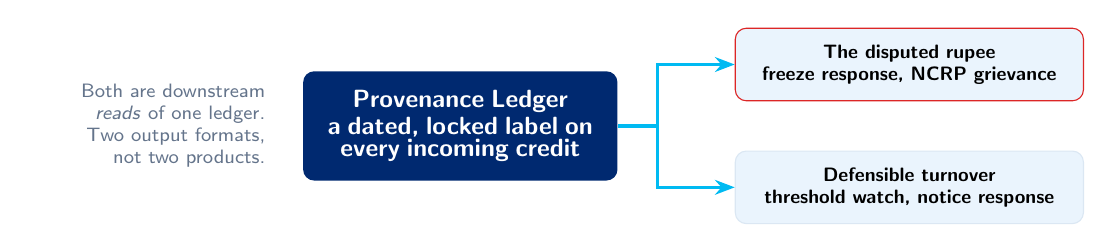
\begin{tikzpicture}[font=\scriptsize]
\node[rounded corners=4pt,fill=navy,text=white,inner sep=7pt,align=center,text width=3.5cm]
  (eng) {\bfseries\small Provenance Ledger\\[0.15em] a dated, locked label on every incoming credit};
\node[rounded corners=4pt,fill=tint,draw=bad,inner sep=6pt,align=center,text width=4.0cm]
  (tax) at ($(eng.east)+(3.7,0.78)$) {\bfseries The disputed rupee\\ freeze response, NCRP grievance};
\node[rounded corners=4pt,fill=tint,draw=hairline,inner sep=6pt,align=center,text width=4.0cm]
  (fra) at ($(eng.east)+(3.7,-0.78)$) {\bfseries Defensible turnover\\ threshold watch, notice response};
\draw[-{Stealth[length=2.5mm]},ptmcyan,line width=1.3pt] (eng.east) -- ++(0.5,0) |- (tax.west);
\draw[-{Stealth[length=2.5mm]},ptmcyan,line width=1.3pt] (eng.east) -- ++(0.5,0) |- (fra.west);
\node[anchor=east,text width=2.9cm,align=right,text=muted] at ($(eng.west)+(-0.35,0)$)
  {Both are downstream \emph{reads} of one ledger. Two output formats, not two products.};
\end{tikzpicture}
\end{center}
\vspace{0.1cm}
\begin{center}
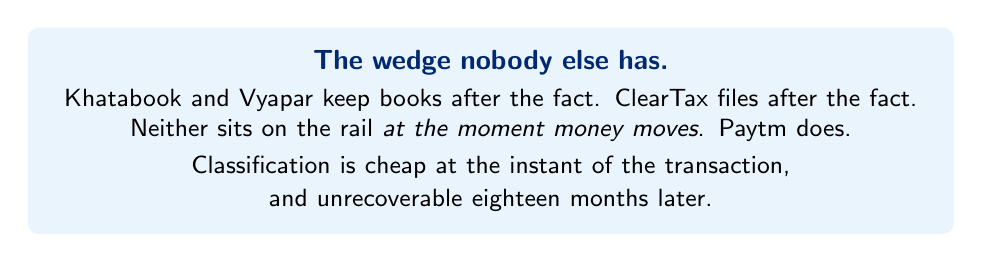
\begin{tikzpicture}\node[rounded corners=4pt,fill=tint,inner sep=8pt,text width=11.2cm,align=center]{
{\bfseries\color{navy}The wedge nobody else has.}\\[0.25em]
\small Khatabook and Vyapar keep books after the fact. ClearTax files after the fact.\\
Neither sits on the rail \emph{at the moment money moves}. Paytm does.\\[0.25em]
\small Classification is cheap at the instant of the transaction,\\ and unrecoverable eighteen months later.
};\end{tikzpicture}
\end{center}
\end{frame}

% ============================================================ 8. THE ENGINE
\begin{frame}{The engine}{Eight labels, and a strict budget on the merchant's attention}
\vspace{0.15cm}
\begin{columns}[T]
\begin{column}{0.45\textwidth}
{\color{navy}\bfseries\small Every incoming credit gets one label}\\[0.4em]
{\scriptsize
\begin{tabular}{@{}ll@{}}
\texttt{taxable\_supply}    & ordinary sale \\
\texttt{exempt\_supply}     & vegetables, milk, loose rice \\
\texttt{refund\_reversal}   & money back from a vendor \\
\texttt{duplicate}          & paid twice, one refunded \\
\texttt{non\_business}      & loan, chit payout, gift \\
\texttt{inter\_account}     & between her own accounts \\
\texttt{personal\_transfer} & from household family \\
{\color{bad}\texttt{unknown}} & {\color{bad}not enough signal, so ask her} \\
\end{tabular}}
\\[0.75em]
{\scriptsize\color{muted}98.6\% are ordinary sales, settled by deterministic rules. The model reasons only about the 1.4\% that need judgement.}
\end{column}
\begin{column}{0.51\textwidth}
\card{6.6cm}{{\bfseries\color{navy}It refuses to guess, and asks instead}\\[0.4em]
\scriptsize Where the rules cannot decide, the credit stays \texttt{unknown} and the agent asks one line, in Kannada, batched daily. A confident wrong label inside an evidence pack is a catastrophe; a question costs one tap.}
\\[0.55em]
\hspace{0.15cm}\begin{minipage}{6.6cm}
{\bfseries\color{navy}\small Budget: at most 3 questions a day.}\\[0.15em]
{\scriptsize\color{muted}Over a simulated year: \hi{189 questions, median 1.3 a day}. Labelling every payment by hand is neither possible nor safe. Ask more than three and the product is dead.}
\end{minipage}
\end{column}
\end{columns}
\end{frame}

% ============================================================ 9. PROVENANCE
\begin{frame}{Why this record cannot be manufactured}{The value of a record is \emph{when} it was made}
\vspace{0.2cm}
\begin{columns}[T]
\begin{column}{0.49\textwidth}
{\scriptsize\color{muted}Anyone can type a history after the freeze arrives. So the ledger is built to make that impossible.}
\\[0.5em]
\card{6.2cm}{{\bfseries\color{navy}The machine's label is never removed}\\[0.3em]
\scriptsize Where the rules cannot decide it stays \texttt{unknown}. Her answer is added \emph{alongside}, marked as her own claim. She cannot overwrite it.\\[0.4em]
{\bfseries\color{navy}She can correct anything, on the record}\\[0.3em]
\scriptsize Any annotation she adds carries the same marking and the date she made it.\\[0.4em]
{\bfseries\color{navy}Append-only and chained}\\[0.3em]
\scriptsize Every entry carries the moment it was recorded. Nothing can be backdated without breaking the chain.}
\end{column}
\begin{column}{0.47\textwidth}
{\scriptsize
\begin{tabular}{@{}L{2.6cm}L{3.5cm}@{}}
\toprule
\multicolumn{2}{@{}l}{\color{navy}\bfseries\small Three questions, one mechanism}\\
\midrule
\sub{Paytm already tags transactions} & That is the consumer app, on money going out, with budgeting labels. Rewritable, and never built to be shown outside Paytm. \\
\addlinespace[0.45em]
\sub{The merchant could lie} & She can. The document says she said it, and says when. She has not laundered a claim into machine output. \\
\addlinespace[0.45em]
\sub{A real mule could use this} & Not retroactively. The history has to already exist, and it has to be mostly backed by bills. \\
\bottomrule
\end{tabular}}
\end{column}
\end{columns}
\end{frame}

% ============================================================ 10. EVIDENCE TIERS
\begin{frame}{The pack says how much each line is worth}{A document that presents everything as equally solid is the one an officer distrusts}
\vspace{0.3cm}
\begin{columns}[T]
\begin{column}{0.55\textwidth}
{\scriptsize\color{muted}Four levels, totalled separately:}
\\[0.45em]
{\scriptsize
\begin{tabular}{@{}rL{5.4cm}@{}}
\grn{1} & \textbf{Backed by a bill}, with items, till and minute \\
\addlinespace[0.35em]
\grn{2} & \textbf{Derived by rule} from the payment's own characteristics \\
\addlinespace[0.35em]
\textcolor{amber}{\bfseries 3} & \textbf{Stated when asked}, on the day the system queried it \\
\addlinespace[0.35em]
\red{4} & \textbf{Added later}, with how long after the payment, and whether before or after the notice arrived \\
\end{tabular}}
\end{column}
\begin{column}{0.41\textwidth}
\vspace{0.1cm}
\ocard{navy}{5.4cm}{{\bfseries\color{navy}The shape does the sorting}\\[0.4em]
\scriptsize A genuine shop's pack is mostly levels 1 and 2.\\[0.3em]
\scriptsize A fabricated one is mostly levels 3 and 4.\\[0.45em]
\scriptsize\color{muted} Nobody has to take our word for which is which.}
\end{column}
\end{columns}
\vspace{0.45cm}
\begin{center}
{\small This makes the pack \emph{more} persuasive, because it stops overclaiming. It is also the honest answer to \qm{what if the merchant is the criminal}: \hi{we sort, we do not advocate.}}
\end{center}
\end{frame}

% ============================================================ 11. THE TEAMMATE
\begin{frame}{The teammate, and where its work goes}{It does not wait to be asked, and it does not send anything on its own}
\vspace{0.15cm}
\begin{columns}[T]
\begin{column}{0.50\textwidth}
{\scriptsize\color{navy}\bfseries Every night, unprompted}\\[0.2em]
{\scriptsize Classifies the day's credits. Queues only what it genuinely cannot settle. Watches the threshold.}
\\[0.5em]
{\scriptsize\color{navy}\bfseries The moment payments start declining}\\[0.2em]
{\scriptsize Detects the freeze. Isolates the disputed credit by reference number \emph{and independently} by amount and date. Pulls the bill behind it. Assembles the pack. Drafts the grievance, citing the SOP and the judgments.}
\\[0.5em]
{\scriptsize\color{bad}\bfseries It stops and hands to a human}\\[0.2em]
{\scriptsize When the evidence does not support release, when the amount is large, and when it is anything other than an ordinary goods sale. Nothing leaves without approval.}
\end{column}
\begin{column}{0.46\textwidth}
\card{6.0cm}{{\bfseries\color{navy}Paytm is the channel}\\[0.4em]
\scriptsize A document handed to a merchant to post somewhere is the weak link. Representations to bank nodal officers go unanswered for months.\\[0.35em]
\scriptsize Paytm is not a stranger to them. It is the regulated PSP, already in the CFCFRMS loop, already answering bank and police requests.\\[0.35em]
\scriptsize \hi{She attests. Paytm answers}, on the channel that already reaches them, inside the SOP's clock.}
\\[0.5em]
{\scriptsize\color{muted}When police ask about a suspect payment, Paytm answers and the merchant is not told. Warning a genuine mule is the worst possible outcome.}
\end{column}
\end{columns}
\vspace{0.1cm}
\hspace{0.05cm}{\scriptsize\bfseries\color{navy}Measured on:}~{\scriptsize time from lien to proportionate release, share of the balance kept operable while the case runs, and share of merchants still transacting thirty days later.}
\end{frame}

% ============================================================ 12. PRODUCT
\begin{frame}{What the merchant sees}
\vspace{-0.1cm}
\begin{center}
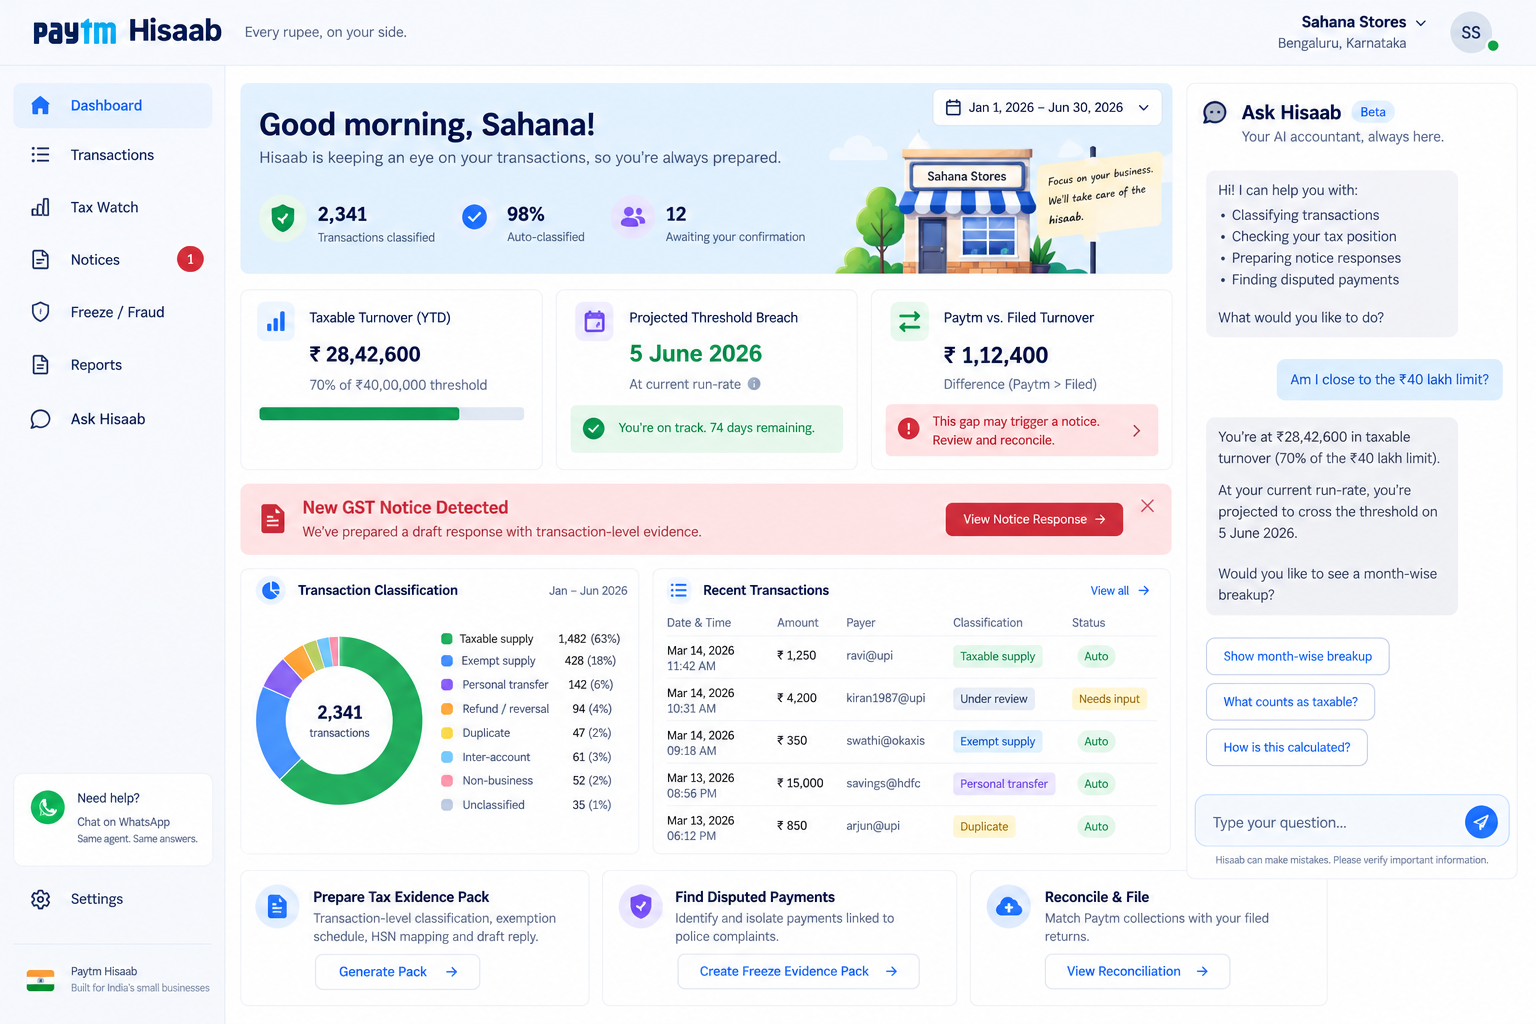
\includegraphics[width=\textwidth,height=0.61\textheight,keepaspectratio]{Paytm-Hisaab_website_look.png}
\end{center}
\vspace{0.1cm}
\hspace{0.05cm}{\scriptsize\color{muted}The default view is the aggregate: how much of her money counts as turnover, how close she is to the threshold, what the packs say. The detail is two taps away and exports on its own, because when the envelope arrives she takes it to a tax practitioner who has never seen this product and has an hour. The same agent runs on WhatsApp, where she actually is.}
\end{frame}

% ============================================================ 13. DEMO / THE FREEZE
\begin{frame}{Demo $\cdot$ The emergency}{Sahana Stores, Jayanagar. Frozen at 09:30, and the supplier payment is due}
\vspace{0.2cm}
\begin{columns}[T]
\begin{column}{0.46\textwidth}
{\scriptsize She sold someone 12kg of onions. That customer was three layers downstream of a fraud victim. She is not named in the FIR, which was filed in another state, and \hi{339 payments} came in that week.}
\\[0.5em]
\card{5.8cm}{{\bfseries\color{navy}The agent isolates it}\\[0.35em]
\scriptsize ₹4,200 on 21 March at 19:47, till POS01. Matched by reference number \emph{and independently} by amount and date.\\[0.3em]
\scriptsize The sale record comes with it: the bill, the items, the till and the minute.}
\end{column}
\begin{column}{0.49\textwidth}
\ocard{amber}{6.1cm}{{\bfseries\color{amber}And the decoy it did not choose}\\[0.35em]
\scriptsize A \emph{second} ₹4,200 that same week, from a regular customer. Listed in the pack, and explicitly \emph{not} named as the disputed one. Only the date separates them.}
\\[0.5em]
{\scriptsize Then it drafts the NCRP and CFCFRMS grievance, asking that only the disputed amount be held, and citing the SOP and the judgments that say so.}
\\[0.5em]
{\scriptsize\color{bad}\bfseries It never asserts that she is innocent.}\\[0.1em]
{\scriptsize\color{muted}Some frozen accounts genuinely are mule accounts. The agent assembles evidence and a human decides.}
\end{column}
\end{columns}
\end{frame}

% ============================================================ 14. DEMO / TAX
\begin{frame}{Demo $\cdot$ The warning, and the notice}{The same ledger, read for the other authority}
\vspace{0.15cm}
\begin{columns}[T]
\begin{column}{0.38\textwidth}
{\scriptsize\color{muted}Replayed as of 31 January:}
\\[0.35em]
\ocard{good}{4.8cm}{{\bfseries\color{ink}\scriptsize\qm{At your current rate you cross ₹40 lakh around {\color{bad}14 March}. You will need to register.}}\\[0.35em]
{\scriptsize\color{muted}\grn{43 days of warning}, and the date is computed, not typed.}}
\\[0.45em]
{\scriptsize\color{bad}\bfseries Its first act on the tax side is telling her to register.}\\[0.1em]
{\scriptsize\color{muted}Before that, on 10 March, thirty-nine credits came in over a weekend and it asked about three. The other thirty-six settled silently, and a ₹23 payment nobody could place was left alone.}
\end{column}
\begin{column}{0.58\textwidth}
{\scriptsize\color{muted}Then the notice arrives, claiming {\color{bad}\bfseries ₹60.98L} of turnover:}
\\[0.3em]
{\scriptsize
\begin{tabular}{@{}lr@{\hskip 1.2em}l@{}}
\multicolumn{2}{@{}l}{\color{navy}\bfseries Aggregate turnover \quad ₹42.2L} & \sub{within \grn{1.6\%} of truth} \\
\midrule
Exempt supplies      & ₹31.3L & \sub{vegetables, loose rice} \\
Taxable supplies     & ₹10.9L & \sub{branded goods, oil, soap} \\
\addlinespace[0.45em]
\multicolumn{2}{@{}l}{\color{navy}\bfseries Not turnover at all \quad ₹18.8L} & \sub{every line traced} \\
\midrule
Refunds, duplicates  & ₹1.0L & \sub{crate returns, double-taps} \\
Loans, chit, gifts   & ₹4.3L & \sub{chit payout, festival gifts} \\
Between her own accounts & ₹7.4L & \sub{top-ups before supplier runs} \\
Family               & ₹6.1L & \sub{spouse, parent, in-law} \\
\bottomrule
\end{tabular}}
\\[0.45em]
{\scriptsize And it says plainly: \hi{the claim is wrong, and you \emph{did} cross ₹40 lakh on 14 March. You must register.}}
\end{column}
\end{columns}
\end{frame}

% ============================================================ 15. NUMBERS
\begin{frame}{What we can actually prove}{One merchant, one year, 13,267 credits, scored against seeded truth}
\vspace{0.45cm}
\begin{columns}[T]
\begin{column}{0.33\textwidth}
\begin{center}\bignum{1.6\%}{error on aggregate turnover\\ (taxable share within 1\%)}\end{center}
\vspace{0.55cm}
\begin{center}\bignum{43 days}{of warning before the\\ threshold crossing}\end{center}
\end{column}
\begin{column}{0.33\textwidth}
\begin{center}\bignum{1.3 a day}{median questions asked.\\ 189 in a year, never over 3}\end{center}
\vspace{0.55cm}
\begin{center}\bignum{zero}{credits left untagged\\ across the whole year}\end{center}
\end{column}
\begin{column}{0.30\textwidth}
\card{3.8cm}{{\bfseries\color{navy}The honest baseline}\\[0.35em]
\scriptsize A 50-line rules-only classifier gets 99.3\% on sale vs not-a-sale, but catches only \red{77.8\%} of non-sale credits.\\[0.3em]
\scriptsize That residue alone puts two eval merchants on the \emph{wrong side} of ₹40L.\\[0.3em]
\scriptsize Closing it is what the agent plus one tap is for.}
\end{column}
\end{columns}
\vspace{0.45cm}
\hspace{0.1cm}{\scriptsize\color{muted}Synthetic data with known ground truth, so accuracy is a measured number rather than a claim. She corrected the agent 52 times that year, and those corrections are the ledger's strongest evidence, not its failures.}
\end{frame}

% ============================================================ 16. STACK
\begin{frame}{How it is built}{Four agents, deterministic skills, and permissions that are part of the product}
\vspace{0.15cm}
\begin{columns}[T]
\begin{column}{0.53\textwidth}
{\scriptsize
\begin{tabular}{@{}L{1.75cm}L{4.7cm}@{}}
\multicolumn{2}{@{}l}{\color{navy}\bfseries\small Autonomous, on a nightly schedule}\\
\midrule
Provenance & proposes a label and a reason for the hard credits \\
Evidence   & assembles packs: freeze response, then exemption schedules \\
\addlinespace[0.6em]
\multicolumn{2}{@{}l}{\color{navy}\bfseries\small Conversational, when she opens it}\\
\midrule
Merchant   & attestation, alerts, Kannada speech in and out \\
Escalation & decides when to stop and route to a human \\
\bottomrule
\end{tabular}}
\\[0.7em]
{\scriptsize\color{muted}\hi{n8n} orchestrates, so every action is a step that can be inspected. \hi{Sarvam} carries the Kannada, because she is behind a counter with one phone. All arithmetic is deterministic Python: versioned, testable, and never model output.}
\end{column}
\begin{column}{0.44\textwidth}
\card{5.7cm}{{\bfseries\color{navy}Permissions are the product}\\[0.4em]
\scriptsize Provenance proposes and \red{never commits}.\\[0.25em]
\scriptsize Only the merchant conversation can record her claim.\\[0.25em]
\scriptsize Evidence is \red{read-only}. The agent that builds the defence cannot edit the evidence.\\[0.25em]
\scriptsize Escalation can \red{halt} anything; a human approves.}
\\[0.5em]
\hspace{0.1cm}\begin{minipage}{5.7cm}{\scriptsize\color{muted}These are enforced, not conventions. A denied call shows up in the trace, and every number in a pack traces back to the credit and the attestation behind it.}\end{minipage}
\end{column}
\end{columns}
\end{frame}

% ============================================================ 17. BUSINESS MODEL
\begin{frame}{Business model}{Four lines, and none of them charge the merchant for being in trouble}
\vspace{0.25cm}
\begin{columns}[T]
\begin{column}{0.48\textwidth}
\card{6.0cm}{{\bfseries\color{navy}1. Retention}\\[0.3em]
\scriptsize A frozen merchant transacts nothing that morning. A frightened one takes the QR down for good. Every merchant kept is retained GMV, a live Soundbox subscription and a lending relationship that still exists. Re-acquiring them costs far more.}
\\[0.35em]
\card{6.0cm}{{\bfseries\color{navy}3. Credit}\\[0.3em]
\scriptsize A merchant with a defensible turnover record is a merchant who can be underwritten. Documented income is the single biggest blocker to small-merchant lending, and lending distribution is Paytm's fastest-growing line.}
\end{column}
\begin{column}{0.48\textwidth}
\card{6.0cm}{{\bfseries\color{navy}2. Migration}\\[0.3em]
\scriptsize Paytm wants vendors off personal VPAs and onto business QRs. What it has never had is a reason the vendor cares about. Karnataka supplied one. Every conversion is a Soundbox rental, a current account and a merchant ID that did not exist before.}
\\[0.35em]
\card{6.0cm}{{\bfseries\color{navy}4. Institutional}\\[0.3em]
\scriptsize Banks and payment companies carry the same duty under the SOP and have none of the data. The bona fide receiver determination is a service Paytm can sell to them.}
\end{column}
\end{columns}
\end{frame}

% ============================================================ 18. CLOSE
\begin{frame}{The line we do not cross}{Accuracy, not minimisation}
\vspace{0.3cm}
\begin{columns}[T]
\begin{column}{0.52\textwidth}
{\scriptsize
$\cdot$\; We \hi{never assert innocence} on a freeze. Some accounts really are mule accounts. We assemble evidence and a human decides.\\[0.5em]
$\cdot$\; We \hi{sort, we do not advocate}. The pack shows which lines are backed by bills and which rest on her word.\\[0.5em]
$\cdot$\; Nothing is \hi{sent to any authority} without human approval.\\[0.5em]
$\cdot$\; We compute what she \hi{genuinely owes} and say so plainly, including \qm{you crossed the threshold, you must register.}\\[0.5em]
$\cdot$\; We \hi{never assert a final liability}. We show the workings and route to a professional.\\[0.5em]
$\cdot$\; We build \hi{nothing} that helps anyone split receipts to stay under a threshold.}
\end{column}
\begin{column}{0.44\textwidth}
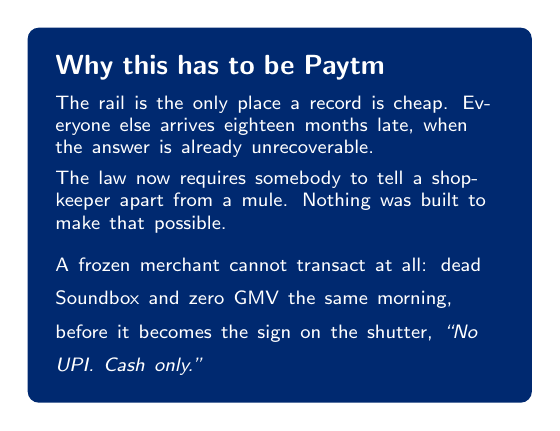
\begin{tikzpicture}\node[rounded corners=4pt,fill=navy,text=white,inner sep=10pt,text width=5.7cm,align=left]{
{\bfseries Why this has to be Paytm}\\[0.45em]
\scriptsize The rail is the only place a record is cheap. Everyone else arrives eighteen months late, when the answer is already unrecoverable.\\[0.45em]
\scriptsize The law now requires somebody to tell a shopkeeper apart from a mule. Nothing was built to make that possible.\\[0.45em]
\scriptsize A frozen merchant cannot transact at all: dead Soundbox and zero GMV the same morning, before it becomes the sign on the shutter, \emph{\qm{No UPI. Cash only.}}
};\end{tikzpicture}
\end{column}
\end{columns}
\vspace{0.4cm}
\begin{center}
{\large\color{navy}\bfseries Paytm Hisaab}\quad{\color{muted}every rupee, on your side.}
\end{center}
\end{frame}

\end{document}
